% ------------------------------------------------------------------------------
% LaTeX template created by
% Iker Algañaraz, May Juarez F., Gastón A. Lozano S., Belén N. Paz
% ------------------------------------------------------------------------------

\documentclass[a4paper,12pt]{article}

% ------------------------------------------------------------------------------
% Packages
% ------------------------------------------------------------------------------
\usepackage{anysize} % Márgenes
\usepackage[hypcap=false, font=small, justification=centering, labelfont=bf]{caption} % Pie de foto/tabla
\usepackage{multicol} % Columnas
\usepackage{amsmath} % Fórmulas matemáticas
\usepackage{amssymb} % Símbolos matemáticos
\usepackage{amsfonts} % Font matemática
\usepackage[utf8]{inputenc} % Facilitar la escritura en español
\usepackage{xcolor} % Color del texto
\usepackage{graphicx} % Figuras
\usepackage[spanish,es-tabla]{babel} % Tipografía del idioma
\usepackage{booktabs} % Separación en tablas
\usepackage{multirow} % Multirow en tablas
\usepackage{hyperref} % Refs como hyperlinks
%\usepackage{biblatex} % Bibliografía automática a partir de base bib

%\usepackage{array}
%\usepackage{verbatim}% Comentarios multilinea
%\usepackage{siunitx} % Unidades del sistema internacional
%\usepackage{fancyhdr} % Personalizar encabezado y pie de pagina
%\usepackage{longtable} % Tablas largas
%\usepackage{blindtext} % Lore ipsum
%\usepackage{soul} % Subrayar
%\usepackage{grffile}
%\usepackage{mathrsfs}

% ------------------------------------------------------------------------------
% Config
% ------------------------------------------------------------------------------
\newenvironment{Figure}
  {\par\medskip\noindent\minipage{\linewidth}}
  {\endminipage\par\medskip}

\providecommand{\abs}[1]{\lvert#1\rvert} % Valor absoluto

\marginsize{2cm}{2cm}{1cm}{2cm} % pkg: anysize

\graphicspath{{./Fotos/}} % pkg: graphicx

\setlength\columnsep{18pt}
\setlength\parskip{4pt} \setlength\parindent{0in}

\title{ Polarización \\ 
\medskip \large Universidad Nacional de Tucumán}
\author{Belén Nahir Paz, May Juarez Ferriol}
\date{}

% ------------------------------------------------------------------------------
% Document
% ------------------------------------------------------------------------------
\begin{document}

\maketitle

\section*{Obtención de luz polarizada}

    \subsection*{Absorción selectiva}

        El Polaroid, ideado por el científico estadounidense Edwin H. Land, es un material diseñado para polarizar la luz mediante el fenómeno del dicroísmo. Este proceso implica la absorción selectiva de luz según su polarización, generando una polarización específica al absorber una de las componentes con mayor intensidad.

        La disminución de la intensidad de la onda incidente en el Polaroid se vincula a su proceso de fabricación. Este material se produce en hojas delgadas de hidrocarburos de cadena larga, estiradas para alinear las moléculas. Al sumergirlas en una solución de yodo, las moléculas se convierten en conductores eléctricos, principalmente a lo largo de las cadenas. Cuando la luz incide con un campo eléctrico paralelo a las cadenas, acelera los electrones, absorbiendo energía y bloqueando la transmisión de luz. En contraste, la luz con un campo eléctrico perpendicular a las cadenas puede pasar, emergiendo polarizada en esa dirección. Este conjunto de procesos explica cómo el Polaroid logra una polarización selectiva y eficaz.

    \subsection*{Reflexión y refracción}

        Este tipo de polarización es un fenómeno común. La luz no polarizada se puede polarizar parcial o completamente por reflexión al incidir en una superficie reflectante entre dos materiales ópticos transparentes. 
        
        En el plano de incidencia, las ondas con el campo eléctrico perpendicular se reflejan con mayor intensidad, parcialmente polarizando la luz en esa dirección. Si modificamos el ángulo de incidencia hasta que el ángulo que se forma entre los rayos reflejado y refractado es de 90°, como en la figura \ref{fig: reflexion}, el rayo reflejado estará totalmente polarizado (con su vector de campo eléctrico paralelo a la superficie), y el rayo refractado estará todavía sólo parcialmente polarizado. El ángulo de incidencia en que se presenta la polarización se conoce como ángulo de polarización $\theta_p$.

        \begin{Figure}
            \centering
            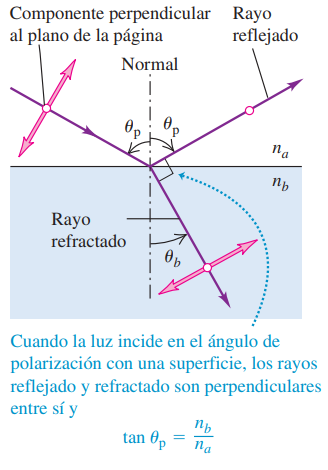
\includegraphics[width=0.35\linewidth]{unnamed.png}
            \captionof{figure}{Polarización por reflexión y refracción}
            \label{fig: reflexion}
        \end{Figure}

        Utilizando la relación $\theta_b=90^\circ-\theta_p$ y la ley de Snell, llegamos a la ley de Brewster:

        \begin{equation}
            tg(\theta_p)=\frac{n_b}{n_a}
        \end{equation}
        
        donde $\theta_p$ se llama ángulo de Brewster.

    \subsection*{Birrefringencia o doble refracción}

        Los materiales birrefringentes, como la calcita y el cuarzo, pertenecen a la categoría de sólidos cristalinos. A diferencia de los sólidos amorfos, como el vidrio, en los cuales la velocidad de la luz es constante en todas las direcciones, en los cristalinos birrefringentes la velocidad de la luz varía según la dirección de propagación y el plano de polarización. Estos materiales se caracterizan por tener dos índices de refracción, lo que les otorga el nombre de birrefringentes o de doble refracción. Cuando la luz no polarizada entra en un material birrefringente, se divide en un rayo ordinario y un rayo extraordinario, ambos con polarizaciones perpendiculares y velocidades distintas. Esta propiedad es especialmente evidente cuando la luz incide en un ángulo al eje óptico, resultando en la separación de los dos rayos polarizados en direcciones diferentes.
    
    \subsection*{Dispersión}

        Cuando la luz incide en cualquier material, los electrones del material absorben y vuelven a enviar parte de la luz. En el caso de las moléculas de gas que conforman el aire, esta absorción y rerradiación de la luz por parte de los electrones es lo que causa que la luz solar que llega a un observador en la Tierra esté parcialmente polarizada. Este efecto, que conocemos como dispersión, se puede observar al mirar directamente al cielo con gafas de sol cuyas lentes están hechas de un material polarizador. Menos luz pasa a través de ciertas orientaciones de las lentes que otras.

        Un haz de luz solar no polarizado que viaja en dirección paralela a la tierra, incide sobre una molécula de uno de los gases que conforman el aire, haciendo vibrar los electrones de esta molécula. Estas cargas vibrantes actúan como cargas vibrantes en una antena. Si el observador está mirando perpendicular a la dirección de propagación de la luz, las oscilaciones verticales de las cargas no envían radiación hacia el observador, por lo que termina viendo luz polarizada horizontalmente.

        No todas las longitudes de onda de la luz se dispersan de la misma manera. Cuando la luz del sol incide en moléculas de gas de diámetro $d$, donde $d \< \<  \lambda$, la intensidad relativa de la luz dispersada varía como $1/\lambda^4$. Esta condición de $d \< \< \lambda$, se cumple para las moléculas de oxígeno y nitrógeno en la atmósfera, cuyos diámetros son cerca de 0.2 mm. Por lo tanto, la luz violeta se va a dispersar más eficientemente que la luz roja, que tiene una longitud de onda mucho mayor.

\section*{Aplicaciones de la luz polarizada}
    
    La fotoelasticidad es como una aplicación de la luz polarizada. Tomamos materiales transparentes y, los sometemos a esfuerzos, vemos cómo la luz que los atraviesa cambia de dirección. La capacidad de observar las variaciones visuales sobre los materiales transparentes nos proporciona información sobre las tensiones y deformaciones experimentadas por el material. Este método, aplicado en el ámbito ingenieril y científico, desempeña un papel crucial en la comprensión del comportamiento estructural bajo condiciones de carga, ya sea compresión o tensión.


\begin{thebibliography}{99}

\bibitem{} R. A. Serway, J. W. Jewett. \emph{Physics for Scientists and Engineers with Modern Physics}, 10th ed. (Cengage, Australia, 2017)

\end{thebibliography}

\end{document}

% ------------------------------------------------------------------------------
% Common references and examples
% ------------------------------------------------------------------------------
% 
% ---------------------------
% Bibliography
% ---------------------------
% \bibitem{} Sears, Zemansky. \emph{Física universitaria}, vol. 2, 14th ed. Pearson Education, 2018.
% \bibitem{} Hecht, Zajac. \emph{Óptica}, 4th ed. Pearson Education, 2003.
% \bibitem{} Serway, Jewett. \emph{Physics for Scientists and Engineers}, vol. 2, 6th ed. Brooks Cole, 2004.
% \bibitem{} Jenkins, White. \emph{Fundamentos de óptica}, 3th ed. Aguilar S.A., 1964.
%
% ---------------------------
% Tables
% ---------------------------
% \begin{Figure}
%     \centering
%
%     \begin{tabular}{c|c}
%         \toprule
%          & \textit{...} \\
%          & \textit{[]} \\
%         \midrule
%         ... & \multirow{2}{*}{$(... \pm ...)$} \\
%         ... & \\
%         ... & \multirow{2}{*}{$(... \pm ...)$} \\
%         ... & \\ \hline
%         ... & $(... \pm ...)$ \\
%         ... & $(... \pm ...)$ \\
%         \bottomrule
%     \end{tabular}
%
%     \captionof{table}{}
%     \label{tab:}
% \end{Figure}
%
% \begin{Figure}
%     \centering
%
%     \begin{tabular}{cc}
%         \toprule
%         \textit{\textbf{... []}} & \textit{\textbf{$... []}}\\
%         \midrule
%         $... \pm ...$ & $... \pm ...$ \\
%         $... \pm ...$ & $... \pm ...$ \\
%         \bottomrule
%     \end{tabular}
%
%     \captionof{table}{}
%     \label{tab:}
% \end{Figure}
%
% ---------------------------
% Figures
% ---------------------------
% \begin{Figure}
%     \centering
%     \includegraphics[width=1\linewidth]{.jpg}
%     \captionof{figure}{}
%     \label{fig:}
% \end{Figure}
%
% ---------------------------
% Equations
% ---------------------------
% \begin{equation}
%     \label{eq:}
%     ...
% \end{equation}